% % \section{Design Process or Methodology Overview }
% % Prepare design process based on objectives and constraints.
% % \section{Preliminary Design or Design (Model) Specification}

% % Present multiple alternative solutions and perform simulations for verification.

% % \section{Data Collection -(If
% % Applicable)}
% % Sources of data and methods of collection.

% % \subsection{Data Cleaning}
% % Techniques used to handle missing values, outliers, and inconsistencies.

% % \subsection{Data Transformation}
% % Methods of normalizing, scaling, or encoding data.

% % \subsection{Data Integration}
% % Combining data from different sources if applicable.
% % \subsection{Data Reduction }
% % Techniques for reducing dimensionality or selecting relevant features.
% % \subsection{Summary of Preprocessed Data}
% % Description of the final dataset used for analysis and design.

% % \section{Implementation of Selected Design}
% % Describe the implementation process.


% % \chapter{Methodology}
% % \label{chap:methodology}

% This chapter presents the proposed methodology for generating region-specific synthetic datasets of adverse driving conditions for autonomous driving pretraining. The objective of the proposed framework is to create a scalable synthetic data factory capable of generating realistic driving scenarios that are difficult, dangerous, or expensive to collect in real-world settings. The generated data are subsequently used to improve the performance of object detection models, particularly for indigenous vehicle classes and uncommon behavioral scenarios frequently observed in South Asian road environments.

% The overall pipeline consists of two generation modes. Mode A generates scene-behavior-consistent static images, whereas Mode B extends the same framework to generate temporally coherent video sequences. Both modes share the same preprocessing and verification stages. Figure~\ref{fig:pipeline} illustrates the complete proposed framework.

% \section{Overview of the Proposed Framework}

% The proposed framework follows a simulation-based learning paradigm, where synthetic samples are generated under controlled conditions while preserving the visual characteristics of real-world driving environments. Instead of synthesizing complete scenes from scratch, the framework modifies real driving images through controlled diffusion-based inpainting. This strategy minimizes the sim-to-real gap by retaining the original road geometry, illumination, and environmental context.

% The complete pipeline consists of the following stages:

% \begin{enumerate}
%     \item Input preparation and scenario definition.
%     \item Scene understanding and structural analysis.
%     \item Prompt construction and behavioral specification.
%     \item Region-of-interest determination and mask generation.
%     \item Multi-ControlNet conditioned SDXL generation.
%     \item Temporal sequence generation for dynamic scenarios.
%     \item Automatic verification and annotation.
%     \item Quality filtering and dataset construction.
%     \item Detector training and evaluation.
% \end{enumerate}

% \section{Input Preparation}

% \subsection{Real Background Collection}

% Real driving scenes serve as the foundation of the generation process. Images are collected from Bangladesh-specific datasets such as BadODD and additional dashcam footage. These images contain authentic road layouts, lighting conditions, infrastructure characteristics, and environmental variations representative of South Asian roads.

% Unlike conventional simulation frameworks that construct entire environments synthetically, the proposed approach preserves the original background pixels. Only selected regions are modified during generation. Consequently, the majority of the generated image remains within the real image distribution.

% \subsection{Class Taxonomy Definition}

% A predefined taxonomy is established to maintain consistency throughout the generation and annotation stages. The taxonomy includes conventional road users as well as region-specific classes, including:

% \begin{itemize}
%     \item Pedestrians,
%     \item Cars,
%     \item Motorcycles,
%     \item Buses,
%     \item Trucks,
%     \item Auto-rickshaws,
%     \item Battery rickshaws,
%     \item Rickshaws,
%     \item Legunas,
%     \item Nosimons,
%     \item Animals,
%     \item Other road obstacles.
% \end{itemize}

% Each class is assigned a fixed identifier compatible with the YOLO annotation format.

% \subsection{LoRA Training for Rare Classes}

% Certain indigenous vehicle categories are absent from the pretrained knowledge of large diffusion models. To address this limitation, Low-Rank Adaptation (LoRA) modules are trained using a small collection of real reference images corresponding to these classes.

% Each LoRA specializes in representing a single concept. During generation, the LoRA weights are loaded into SDXL, enabling the model to synthesize region-specific objects while preserving the general visual capabilities of the base model.

% \section{Scene Understanding}

% Before image generation, the structural characteristics of the scene are extracted using pretrained vision models.

% \subsection{Semantic Segmentation}

% A SegFormer network is employed to generate semantic segmentation maps of the input background image. The segmentation output identifies important scene components such as road surfaces, sidewalks, vegetation, buildings, and existing vehicles.

% These segmentation maps provide spatial context regarding where newly inserted agents may plausibly appear.

% \subsection{Depth Estimation}

% Depth information is estimated using a monocular depth estimation model. The resulting depth map provides relative distance relationships within the scene.

% The depth representation ensures that generated objects maintain realistic scale, perspective, and spatial consistency with respect to the original environment.

% \section{Scenario Definition and Prompt Construction}

% Behavioral realism is introduced through scenario templates.

% Each template specifies:

% \begin{itemize}
%     \item The target agent category,
%     \item The behavioral state,
%     \item The environmental context,
%     \item The interactions expected from surrounding traffic.
% \end{itemize}

% For example, a jaywalking scenario may describe:

% \begin{quote}
% ``A pedestrian crossing between moving vehicles during congested urban traffic.''
% \end{quote}

% Pose descriptions are incorporated directly into the textual prompt. These prompts are subsequently encoded by SDXL's text encoder and influence the generated content through cross-attention mechanisms.

% \section{Response Zone Generation}

% To preserve scene consistency, geometric constraints are introduced through response zones.

% Response zones define regions within which particular objects are allowed to appear. Examples include:

% \begin{itemize}
%     \item Pedestrian crossing areas,
%     \item Vehicle stopping regions,
%     \item Safe gaps around traffic officers,
%     \item Lane-adjacent regions for cut-in vehicles.
% \end{itemize}

% The coordinates associated with these zones do not directly constrain SDXL. Instead, they determine where editing masks are placed and influence the textual descriptions used during generation.

% \section{Context-Aware Mask Generation}

% Binary masks are generated to specify which image regions are allowed to be modified.

% Formally, the mask function is defined as:

% \[
% M(x,y)=
% \begin{cases}
% 1, & \text{if pixel } (x,y) \text{ belongs to editable regions,}\\
% 0, & \text{otherwise.}
% \end{cases}
% \]

% Pixels assigned a value of one are regenerated by SDXL, whereas pixels assigned a value of zero remain unchanged.

% The mask includes not only the target object location but also surrounding contextual regions such as shadows, contact surfaces, and neighboring traffic participants to ensure seamless integration.

% \section{Multi-ControlNet Conditioning}

% ControlNet modules are employed to preserve the structural characteristics of the original scene.

% Three conditioning signals are used:

% \begin{enumerate}
%     \item Canny edge maps,
%     \item Depth maps,
%     \item Semantic segmentation maps.
% \end{enumerate}

% The Canny representation preserves object boundaries and lane structures. The depth representation enforces spatial realism, while semantic segmentation constrains objects to contextually valid regions.

% These conditioning signals are injected into the SDXL denoising process through ControlNet residual connections.

% \section{Mode A: Scene-Behavior-Consistent Still Generation}

% Mode A produces static synthetic images using a two-pass inpainting strategy.

% \subsection{Pass 1: Agent Placement}

% During the first generation stage, the mask covers only the target agent region.

% The original background image, the corresponding control maps, the scenario prompt, and the relevant LoRA weights are provided to the SDXL inpainting pipeline.

% The diffusion process modifies only the masked region, generating the desired agent while preserving the remainder of the image.

% \subsection{Pass 2: Environmental Response Generation}

% The output of Pass 1 serves as the input to the second stage.

% A new mask is generated covering neighboring traffic participants and interaction zones. The previously generated agent remains outside the editable region.

% The prompt is updated to describe how surrounding traffic should respond to the inserted event.

% Examples include:

% \begin{itemize}
%     \item Vehicles slowing down,
%     \item Formation of safety gaps,
%     \item Traffic queues,
%     \item Avoidance maneuvers.
% \end{itemize}

% This two-stage strategy guarantees that the primary agent remains unchanged while the surrounding environment adapts accordingly.

% \section{Mode B: Temporal Corner-Case Generation}

% Although SDXL produces only static images, temporal scenarios are essential for modeling behavioral evolution.

% Mode B extends Mode A through keyframe interpolation.

% \subsection{Keyframe Generation}

% Two keyframes are generated independently using the Mode A pipeline.

% The initial keyframe represents the beginning of the event, whereas the final keyframe depicts the completed scenario.

% Examples include:

% \begin{itemize}
%     \item A pedestrian standing at the roadside versus crossing the road,
%     \item A traffic officer lowering versus raising a hand signal,
%     \item Vehicles before and after braking.
% \end{itemize}

% \subsection{Video Interpolation}

% The generated keyframes are subsequently passed to the Wan First-Last-Frame-to-Video (FLF2V) model.

% Wan synthesizes temporally coherent intermediate frames that connect the two endpoints.

% Unlike traditional frame interpolation algorithms, Wan employs diffusion-based generation to produce plausible motion trajectories while maintaining visual consistency.

% The resulting clips capture gradual behavioral transitions suitable for video-based learning tasks.

% \section{Automatic Verification and Annotation}

% To eliminate manual labeling requirements, the generated outputs undergo automated verification.

% \subsection{Grounding DINO Detection}

% Grounding DINO performs open-vocabulary detection using textual descriptions of target classes.

% Bounding boxes corresponding to expected objects are identified.

% Images in which required objects cannot be detected are discarded.

% \subsection{SAM Refinement}

% The Segment Anything Model (SAM) generates precise segmentation masks for detected objects.

% Bounding boxes are recalculated from the refined masks, ensuring that annotations correspond to actual object extents rather than planned placements.

% \subsection{Temporal Tracking}

% For video sequences, Grounded SAM 2 propagates masks across consecutive frames.

% This procedure provides consistent annotations throughout the generated clip without repeated detection.

% \section{Behavior Consistency Validation}

% Visual realism alone does not guarantee behavioral plausibility.

% Therefore, additional rule-based validation procedures are introduced.

% The following constraints are enforced:

% \begin{itemize}
%     \item No overlap between pedestrians and vehicles,
%     \item Presence of safety gaps around designated agents,
%     \item Ground contact consistency,
%     \item Agreement between agent behavior and surrounding traffic responses.
% \end{itemize}

% Samples violating these conditions are removed from the dataset.

% \section{Automatic YOLO Annotation}

% Validated bounding boxes are converted into YOLO annotation format.

% Each object instance is represented as:

% \[
% (class\_id,\;x_{center},\;y_{center},\;width,\;height),
% \]

% where all coordinates are normalized relative to image dimensions.

% Consequently, generation and annotation occur simultaneously without requiring human intervention.

% \section{Quality Assessment and Filtering}

% Distribution-level quality assessment is performed prior to dataset integration.

% For image datasets, Fréchet Inception Distance (FID) and Kernel Inception Distance (KID) are employed to evaluate similarity between synthetic and real distributions.

% For video sequences, Fréchet Video Distance (FVD) is utilized.

% Frames exhibiting excessive redundancy or low realism scores are excluded.

% This stage ensures that the final dataset maintains both diversity and visual fidelity.

% \section{Detector Training}

% The resulting dataset is combined with real-world annotated samples.

% YOLO-based object detectors are trained using a two-stage strategy.

% Initially, models undergo pretraining using the generated synthetic data.

% Subsequently, fine-tuning is performed using real Bangladeshi driving datasets.

% This approach allows the detector to learn rare scenarios during pretraining while adapting to the statistical characteristics of real environments during fine-tuning.

% \section{Evaluation Protocol}

% Performance evaluation is conducted using a fixed real-world validation set.

% The primary metric is mean Average Precision (mAP), including both mAP@0.50 and mAP@0.50:0.95.

% Per-class Average Precision values are also reported, with particular emphasis on indigenous vehicle categories and rare behavioral scenarios.

% The proposed approach is compared against a baseline trained exclusively on real data.

% Improvements obtained through synthetic pretraining demonstrate the effectiveness of the proposed data generation framework.

% \section{Iterative Refinement}

% The proposed methodology incorporates a feedback mechanism.

% Generation parameters including prompts, mask sizes, ControlNet weights, and behavioral templates are adjusted based on verification outcomes and detector performance.

% This iterative process continuously improves both dataset quality and downstream detection performance.

% \section{Summary}

% The proposed methodology introduces a region-specific synthetic data generation framework designed to address the scarcity of adverse driving scenarios in South Asian road environments. Real backgrounds provide environmental realism, ControlNet-conditioned SDXL inpainting generates behaviorally consistent events, Wan produces temporally coherent video sequences, and automated verification ensures annotation quality. The resulting dataset enables efficient pretraining of object detection models while significantly reducing the costs and risks associated with real-world data collection.





\section{Methodology Overview}

Our proposed methodology develops a region-specific synthetic data generation framework for producing realistic adverse driving scenarios, with the aim of pretraining autonomous vehicle detectors on conditions that real-world collection cannot easily provide. The central challenge it addresses is the persistent scarcity of annotated data representing South Asian traffic — particularly scenarios involving indigenous vehicle classes, unusual traffic behaviours, and hazardous road events. Four guiding constraints shape the entire design: visual realism must be maintained, the sim-to-real gap minimised, annotations produced automatically, and the dangers of collecting genuinely hazardous footage on real roads avoided.
The pipeline operates in two complementary modes — a still-image generation pipeline (Mode A) and a temporal scenario generation pipeline (Mode B). Across both modes, Stable Diffusion XL (SDXL) \cite{rombach2022latentdiffusion,podell2024sdxl} is the sole generator of pixels; it operates in exactly two places: the two-pass inpaint in Mode A, and the generation of start and end keyframes in Mode B. Everything else in the pipeline exists to serve SDXL or to check its output. The prompt, mask, and three control images are all preparation. The verification, labelling, and quality filtering stages are all downstream. ControlNet does not generate anything independently; it feeds structural constraints into SDXL's denoising process so that what gets painted respects the original scene geometry. Wan is a separate model entirely, brought in only for the motion generation step in Mode B. The methodology begins with real driving backgrounds drawn from BadODD and supplementary dashcam footage. These backgrounds supply authentic road geometry, illumination conditions, infrastructure characteristics, and existing environmental context, forming the structural foundation of every generated frame.
To introduce region-specific concepts that SDXL's pretrained weights do not contain, Low-Rank Adaptation (LoRA)\cite{hu2022lora} modules are trained using small reference image sets corresponding to indigenous We only train a LoRA where the base model genuinely falls short — each locally rare vehicle class that SDXL cannot render convincingly gets its own adapter, and anything the base model already handles well is left alone.
Before generation, scene understanding is applied to each background using two pretrained networks. SegFormer reads the background and produces a colour-coded map of what each region is — road surface, vehicle, sky, sidewalk, and so on. Depth Anything produces a matching per-pixel depth estimate, giving us the spatial distances and perspective foreshortening we need to place agents convincingly. Crucially, these three outputs the segmentation map, the depth map, and the edge map serve as control images for ControlNet\cite{zhang2023controlnet}; they constrain the structure of the generated content but do not contribute to the text prompt.
Behavioural scenarios are defined through template-based prompt generation. Scenario templates specify the target event, the participating agents, and their associated behavioural states; each behavioural state is translated into concrete prompt words that directly determine what SDXL paints. Simultaneously, response zones are computed through geometric reasoning to identify plausible placement regions within the scene. These zones have two roles: they determine where the binary mask is drawn, and they inform the wording of the second-pass prompt but they are never passed as numeric coordinates to SDXL. Context-aware binary masks are then constructed from the zone geometry to define exactly which regions of the image may be modified during inpainting.
The prepared prompts, masks, and control images are supplied to a Multi-ControlNet\cite{zhang2023controlnet} conditioned SDXL inpainting framework. ControlNet acts as an adapter — feeding the structural maps into SDXL's UNet — rather than as an independent generator. In Mode A, a two-pass inpainting strategy is employed. The first pass synthesises the primary agent within the masked region, repainting only that area while leaving all other real pixels untouched. The second pass then receives the first pass's output as its input image; the mask is repositioned over the surrounding traffic area, and the previously placed agent — now sitting beneath a black, preserved region of the mask — remains completely intact while SDXL reshapes the nearby traffic behaviour to match the scenario. The Canny edge map, depth map, and segmentation map are all derived from the original background and computed once; they are reused in both passes without modification.
In Mode B, the Mode A pipeline is executed twice on the same background to produce start and end keyframes that differ only in the agent's behavioural state — the start frame captures the agent before the event and the end frame captures the resolved state. Wan 2.2 First-Last-Frame-to-Video (FLF2V))\cite{wan2025wan} then generates the intermediate frames connecting the two endpoints. Unlike classical frame interpolation methods, which blend pixels between two frames and introduce ghosting on real motion, Wan is a video diffusion model that synthesises physically plausible in-between content — generating motion states that neither keyframe contains. The resulting clip captures the agent across many positions, scales, and poses, yielding dozens of varied labelled frames from a single keyframe pair.
Generated outputs are verified automatically using Grounding DINO\cite{liu2024groundingdino}, which performs open-vocabulary detection to confirm the presence of intended objects. For video sequences, Grounding DINO seeds detection on frame zero and Grounded SAM 2 then propagates that segmentation mask forward and backward through every frame in the clip, providing consistent object boundaries at each timestep without re-detecting per frame. For still images, SAM refines the detected boundaries by tracing the agent's actual pixel outline rather than relying on the rough placement box used during scene planning; the final annotation box is fitted around that outline, ensuring labels reflect where the agent genuinely is rather than where it was intended to be. After the annotation pass, a set of simple geometric rules screens each generated frame: the inserted agent cannot physically occupy the same space as a nearby vehicle, a clear gap must exist around it, its base must sit on the road rather than floating above it, and the traffic state visible in the surrounding scene must be consistent with whatever the agent is supposed to be doing. Frames that fail any check are discarded before they can pollute the annotation pool. What passes gets quality-filtered using FID, KID, and FVD, and whatever clears those thresholds is merged with real-world data for training and evaluation. When too many outputs fail verification, or when evaluation numbers on target classes are not improving, we go back and adjust the prompts, zone placements, mask boundaries, or ControlNet weights, then run the whole thing again. The loop closes when the data quality reaches the level we need. The complete methodology is illustrated in the proposed pipeline shown in Figure 3.1.\\
\begin{figure}[h]
    \centering
    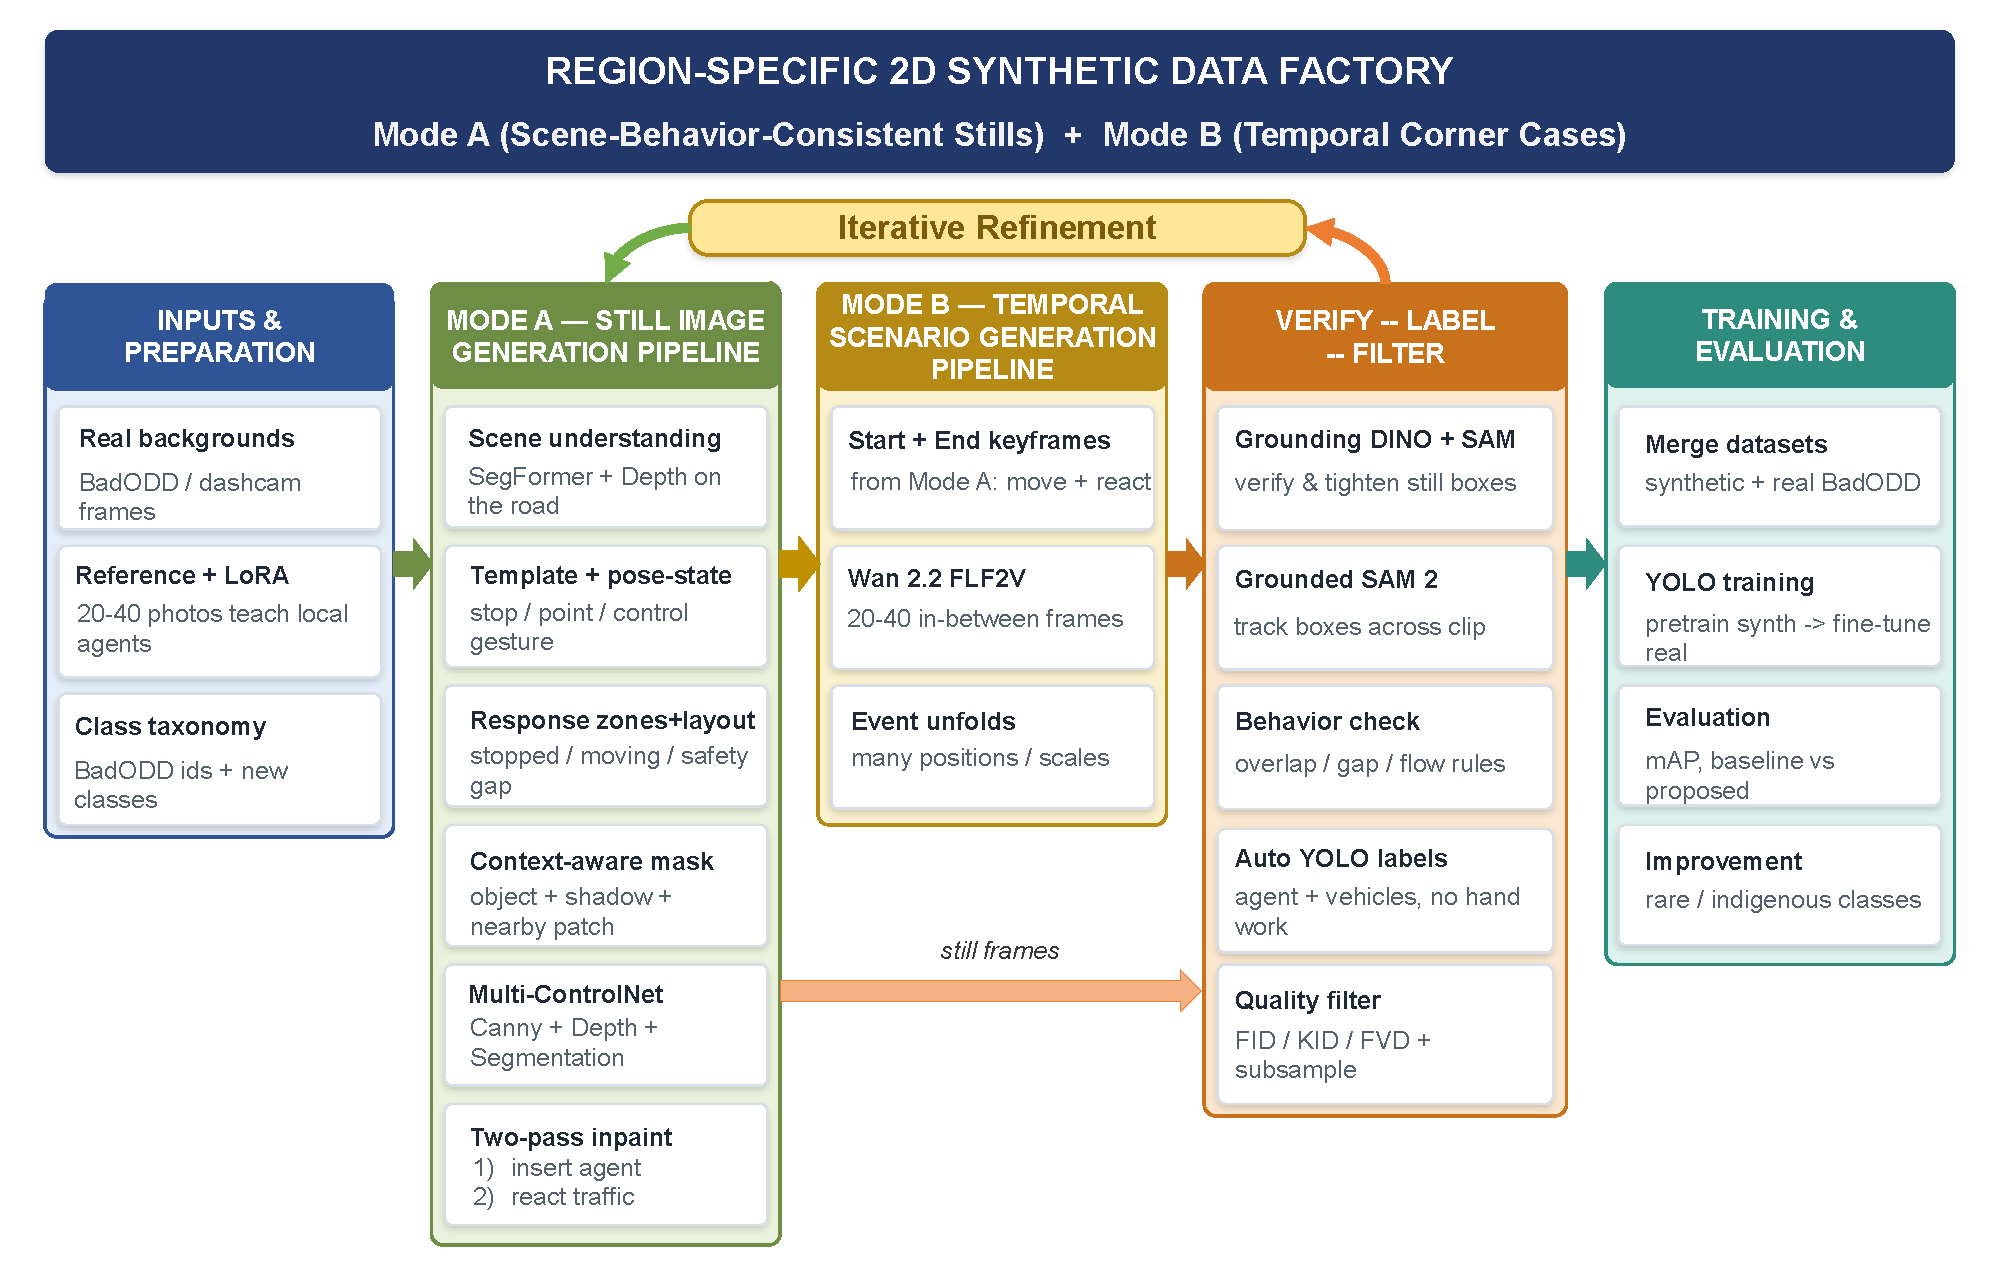
\includegraphics[width=15cm]{images/Methodology.pdf}\\
    \caption{Methodology}
    \label{fig:sample}
\end{figure}
\section{Preliminary Design Specification}

Several design alternatives were evaluated before arriving at the proposed framework.Traditional simulation environments such as CARLA provide physically grounded scenarios and automatic annotations; however, they require significant effort to create assets representative of South Asian traffic the indigenous vehicles, road markings, and infrastructure that define the target domain. Moreover, the visual appearance of simulated environments typically differs substantially from real dashcam imagery, compounding the sim-to-real problem rather than reducing it. Generative text-to-image pipelines were also investigated. While fully generative pipelines are able to create a variety of scenarios, the creation of an entire frame from scratch leads to unrealistic road geometry, inconsistency of spatial layout, and inability to maintain precise object relations issues becoming even more critical given the spatial nature of the traffic intersection. In order to solve the problems inherent in both sets of methods, a hybrid generation pipeline was designed. Instead of creating something from scratch, we began with actual photographs and then edited those photographs. All the frames in our pipeline begin as photographs taken by a dashcam; the role of diffusion-based inpainting is limited to adding a new agent or event at the specified location. We have selected SDXL for our generation purposes due to its superiority in quality and ControlNet compatibility. ControlNet adapters receive such inputs as Canny edges, depth maps, and segmentation maps, all of which are extracted from the source photograph. This helps us to stick to actual scene geometry rather than generating something fake-looking.
LoRA modules address the indigenous concept gap: each rare class that the base SDXL model fails to represent adequately gets its own targeted adapter trained on 20–40 reference images, while common vehicle types SDXL already knows need none. The two-pass inpainting strategy was chosen over single-pass generation because it decouples agent placement from environment adjustment and the inserted agent is locked in place in the first pass while the surrounding traffic is independently modified in the second.
For temporal generation, Wan 2.2 FLF2V was chosen over classical frame interpolation methods such as RIFE or FILM. Classical approaches work by blending pixels between two endpoint frames and introduce ghosting wherever significant real motion is involved. Wan, by contrast, is a video diffusion model that generates physically plausible intermediate content, producing motion states that neither keyframe contains, such as a limb mid-gesture or a wheel mid-turn which is what makes the resulting sequences look genuinely natural rather than blended.


The final design therefore consists of the following components:

\begin{itemize}
    \item Real-world driving backgrounds,
    \item Scenario-specific prompt generation,
    \item LoRA-based indigenous concept adaptation,
    \item SegFormer\cite{xie2021segformer} semantic segmentation,
    \item Monocular depth estimation,
    \item Context-aware mask generation,
    \item Multi-ControlNet conditioned SDXL inpainting,
    \item Wan FLF2V video generation,
    \item Grounding DINO\cite{liu2024groundingdino} and SAM verification,
    \item Automatic YOLO annotation generation.
\end{itemize}

Each of those choices addresses a specific failure mode in the alternatives we considered together they produce a pipeline that is realistic enough to train on, controllable enough to target specific rare classes, and scalable enough to produce a dataset of meaningful size without manual annotation effort.\\


\section{Data Collection }

% The framework draws on both real-world and synthetic data. Real-world images provide the structural foundation on which synthetic modifications are applied.
% The primary real-world source is the Bangladeshi Autonomous Driving Object Detection Dataset (BadODD\cite{saha2024bnvd}). Additional driving footage from dashboard cameras may be incorporated to broaden environmental diversity. Together, these sources provide authentic representations of South Asian road infrastructure, vehicle distributions, lighting conditions, and traffic behaviours.
Our dataset is not purely synthetic but real imagery underpins everything. The actual road surfaces, vehicle distributions, and lighting conditions in every generated frame come from genuine dashcam footage, with BadODD\cite{saha2024bnvd} as the primary source.
For LoRA training, small reference image sets are gathered for each indigenous vehicle category and rare traffic agent in scope. Twenty to forty representative images are typically sufficient to adapt SDXL to a given local concept. Because each rare class that the base SDXL model cannot handle requires its own LoRA while common classes need none, the collection effort is concentrated precisely on the gap classes rather than spread across the whole taxonomy.
The synthetic component of the dataset is generated automatically by the diffusion-based pipeline. Scenario templates are paired with diverse real backgrounds to produce a wide range of adverse driving conditions that would be either too dangerous or logistically impractical to capture from real roads.


\subsection{Data Cleaning}

Real-world datasets undergo a cleaning pass before use. Duplicate images, severely corrupted files, and visually unusable samples are removed from the dataset.
For the reference sets used in LoRA training, images with excessive occlusion, poor visibility, or incorrect class representation are excluded to ensure the adapter learns the intended concept cleanly.
After synthetic generation, an additional quality control pass is applied. Grounding DINO verification identifies cases where intended objects were not successfully produced, and those samples are automatically discarded. Geometry-based behaviour checks further eliminate unrealistic outputs involving object overlap, floating agents, or inconsistent traffic responses.


\subsection{Data Transformation}

Several transformation steps occur at different points in the pipeline.
During scene understanding, semantic segmentation maps and depth maps are extracted from each original background. Canny edge detection\cite{canny1986edge} is also applied to obtain structural edge representations of the scene.
Prompt transformation converts predefined behavioural states into textual descriptions appropriate for SDXL conditioning. Context-aware masks are converted into binary representations marking editable and non-editable regions.
For detector training, verified object annotations are expressed in YOLO-compatible format, consisting of normalised centre coordinates and bounding box dimensions.


\subsection{Data Integration}

The final training dataset is assembled by combining multiple sources.
Real-world images from BadODD are combined with synthetic still images generated through Mode A. Temporal sequences generated through Mode B are incorporated by extracting verified frames at predefined intervals.
Annotations from Grounding DINO and SAM on the synthetic side are merged directly with the existing real-world labels from BadODD to form a single YOLO-format training split. The detector sees both authentic road conditions and the rare synthetic scenarios in the same batch neither source alone would cover the full range of what we need it to learn.


\subsection{Data Reduction}

% Data reduction procedures are applied to improve training efficiency and remove redundancy.
% For Mode B video sequences, temporal subsampling selects representative frames at fixed intervals to prevent near-duplicate frames from dominating the dataset.
% Implicit feature reduction also occurs through the use of segmentation maps, depth representations, and control images, each of which retains only the structural information relevant to generation.
% Quality filtering based on Fréchet Inception Distance (FID)\cite{heusel2017fid}, Kernel Inception Distance (KID), and Fréchet Video Distance (FVD) further reduces the dataset by removing samples that exhibit poor realism or significant distributional deviation from the real-world domain.
If left unchecked, the Mode B sequences would flood the dataset with near-identical frames. We prevent that by subsampling at fixed intervals, picking one representative frame every N timesteps rather than keeping everything Wan produces. The control images act as an implicit reduction on top of that segmentation maps, depth representations, and Canny edges carry only the structural content that matters for generation, stripping out irrelevant variation. FID\cite{heusel2017fid}, KID, and FVD scores then provide a distributional checkpoint: any sample that sits too far from the real-world statistics gets dropped before training begins.


\subsection{Summary of Preprocessed Data}

% The final preprocessed dataset consists of real and synthetic samples in YOLO format\cite{jocher2023yolov8}. Each sample pairs an RGB image with an annotation file specifying object classes and normalised bounding box coordinates. The dataset covers conventional vehicle categories, pedestrians, and indigenous South Asian traffic participants such as rickshaws and auto-rickshaws. The synthetic component enriches it with diverse adverse driving conditions — including uncommon traffic interactions and hazardous scenarios — all grounded in the visual characteristics of real Bangladeshi roads. The resulting dataset provides both environmental diversity and behavioural variability while maintaining consistency with the visual domain of the real-world source material.
What comes out the other end is a YOLO-format dataset\cite{jocher2023yolov8} where every sample is an RGB image paired with a text file of class labels and normalised bounding boxes. The class set covers standard driving categories alongside the local classes that motivated this project: rickshaws, auto-rickshaws, and the other indigenous South Asian vehicle types that standard benchmarks have never included. The synthetic portion is what gives the dataset its behavioral range dangerous close-contact scenarios and adverse driving conditions that genuine dashcam footage would rarely capture by chance are all present, but they sit within the visual domain of real Bangladeshi roads rather than looking like they came from a rendering engine.

\section{Implementation of Selected Design}

Implementation begins by selecting a real driving background from the prepared dataset. SegFormer and Depth Anything are applied to produce a semantic segmentation map and a depth map respectively, while Canny edge detection is run on the original background to extract a structural edge representation of the scene. All three control images the segmentation map, the depth map, and the Canny edge map are derived from the original background and computed once; they are reused in both inpainting passes without any modification. Concurrently, scenario templates generate textual prompts describing the intended traffic event.
Response zones are defined through geometric reasoning to identify plausible locations for object insertion. These zones determine both where the binary mask is drawn and how the second-pass prompt is worded. Binary masks for the identified zones are subsequently generated using OpenCV.
The prompt, mask, segmentation map, depth map, and Canny edge map are supplied to a Multi-ControlNet conditioned SDXL inpainting framework. During the first inpainting pass, the primary agent is synthesised within the selected region; SDXL repaints only the masked area while all other real pixels remain untouched. In the second pass, the output of the first pass becomes the new input image, and the mask is repositioned over the surrounding traffic area rather than the agent. The previously placed agent now falls beneath a black, preserved region of the mask and is kept completely intact while SDXL adjusts the nearby traffic behaviour to match the scenario.
For temporal scenarios, the still-image pipeline is executed twice on the same background to produce start and end keyframes. The two keyframes differ only in the agent's behavioural state: the start frame captures the agent before the event and the end frame captures the resolved state. Wan 2.2 FLF2V receives the two keyframes along with a short motion prompt and generates the intermediate frames connecting them. Unlike classical frame interpolation, which merely blends pixels and introduces ghosting on real motion, Wan synthesises genuinely plausible in-between content rendering motion states that neither endpoint frame contains. The resulting clip provides the agent at many positions, scales, and poses across the sequence, yielding dozens of varied labelled frames from a single keyframe pair.
Following generation, Grounding DINO performs open-vocabulary detection to verify the presence of intended objects. For video sequences, detection is seeded on frame zero and Grounded SAM 2 then propagates the resulting segmentation mask through every frame of the clip, supplying consistent object boundaries at each timestep without re-detecting per frame. For still images, the rough placement box used during inpainting planning is not necessarily where the agent ended up SDXL paints within the masked region at its own scale and exact position. SAM corrects for this by tracing the actual pixel boundary of the agent; the annotation box is then drawn around that trace, so the label reflects where the agent genuinely is rather than where the mask was drawn. Finally, a number of geometric constraints are enforced on the output that is no spatial overlap with other vehicles, a definite safe distance around the agent,
ground contact verification, and matching traffic situation according to the behavior
of the agent. Those frames which fail one constraint or another are removed at once,
and the successful examples are automatically annotated into YOLO format. Finally,
distribution metrics (FID, KID, and FVD) are calculated, and those which stray too
far from the real distribution are removed from the set. After this stage, the dataset
is mixed with BadODD and trained. Our method of training comes in two phases. The
first trains only with synthetic data, allowing the model to learn the difficult
indigenous classes and adverse situations without ever seeing an actual image. The second phase is used to fine-tune using actual BadODD video data. When outputs from the verification pass or the quality metrics fall short too many rejections, or mAP on target classes not moving we revisit the generation settings, adjust, and run again. Final performance is measured in mAP and per-class AP, with the indigenous vehicle categories given particular weight since those are the classes the whole project exists to address.